\normaltrue \difficilefalse \tdifficilefalse
\correctionfalse

%\UPSTIidClasse{11} % 11 sup, 12 spé
%\newcommand{\UPSTIidClasse}{11}

\exer{Identification $\star$ \label{B2:06:506}}
\setcounter{question}{0}\marginnote{\xpComp{SLCI}{07}}%\UPSTIcompetence[2]{B2-06}
\index{Compétence B2-06}
\index{Identification}
\index{Identification Bode}
\index{Identification fréquentielle}
\index{Réponse fréquentielle}

\ifcorrection
\else
\marginnote{\textbf{Pas de corrigé pour cet exercice.}}
\fi


\ifprof 
\else
Soit la réponse fréquentielle ci-contre \ref{B2:06:506:01:fig}}.
\begin{marginfigure}
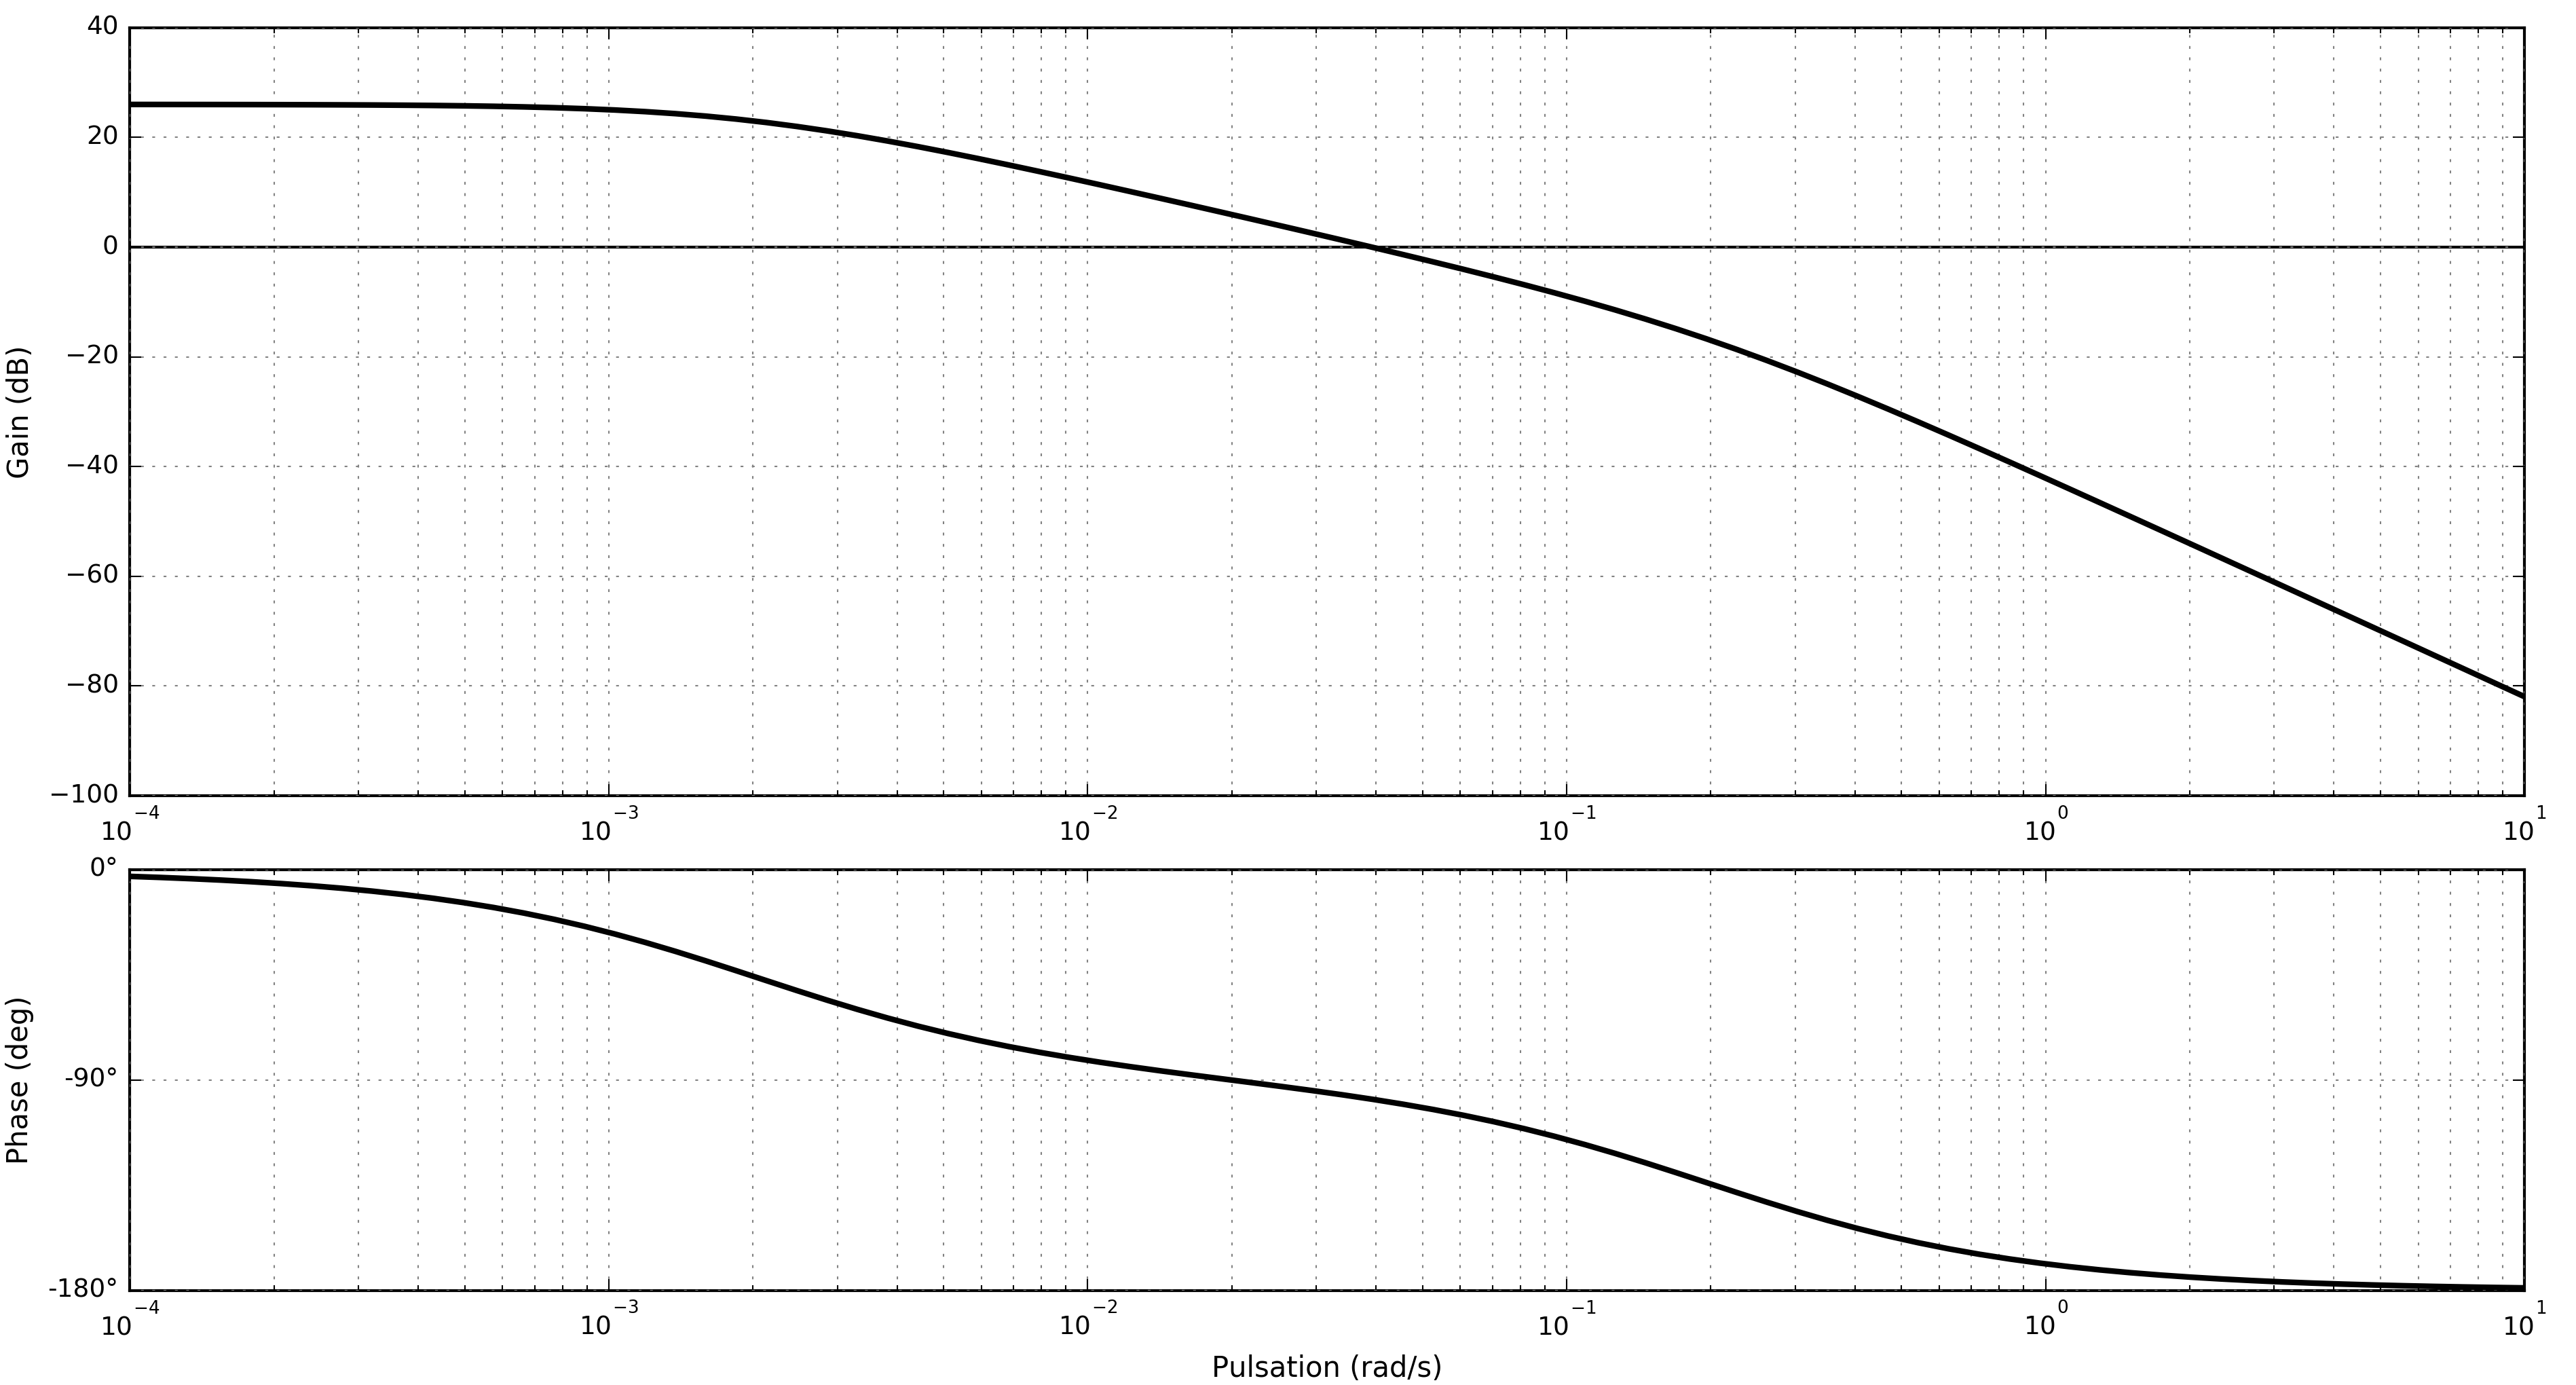
\includegraphics[width=\linewidth]{506_01}
\caption{Diagramme 1 \label{B2:06:506:01:fig}}
\end{marginfigure}
\fi

\question{Déterminer la fonction de transfert du système.}

\ifprof
La pente est de \SI{0}{dB} par décade en basse fréquence et de \SI{-40}{dB} par décade en haute fréquence. Il n'y a pas de résonance. On peut donc faire l'hypohèse qu'il s'agit d'un système d'ordre 2 de la forme $H(p)=\dfrac{K}{\left( 1+\tau_1 p\right)\left( 1+\tau_2 p\right)}$.


Sur la courbe de phase, on mesure des pulsations de cassure à \SI{0,002}{rad/s} et de \SI{0,2}{rad/s} respectivement pour des déphasages de $-90$ et $-180$ degrés. Les constantes de temps sont donc $\tau_1 =\dfrac{1}{0,002}= \SI{500}{s}$ et $\tau_2 =\dfrac{1}{0,2} = \SI{5}{s}$.

Le gain en basse fréquence est de \SI{25}{dB} soit $K = 10^{25/20}=17,8$.


Au final, $H(p)=\dfrac{17,8}{\left( 1+500 p\right)\left( 1+ 5p\right)}$.

\begin{center}
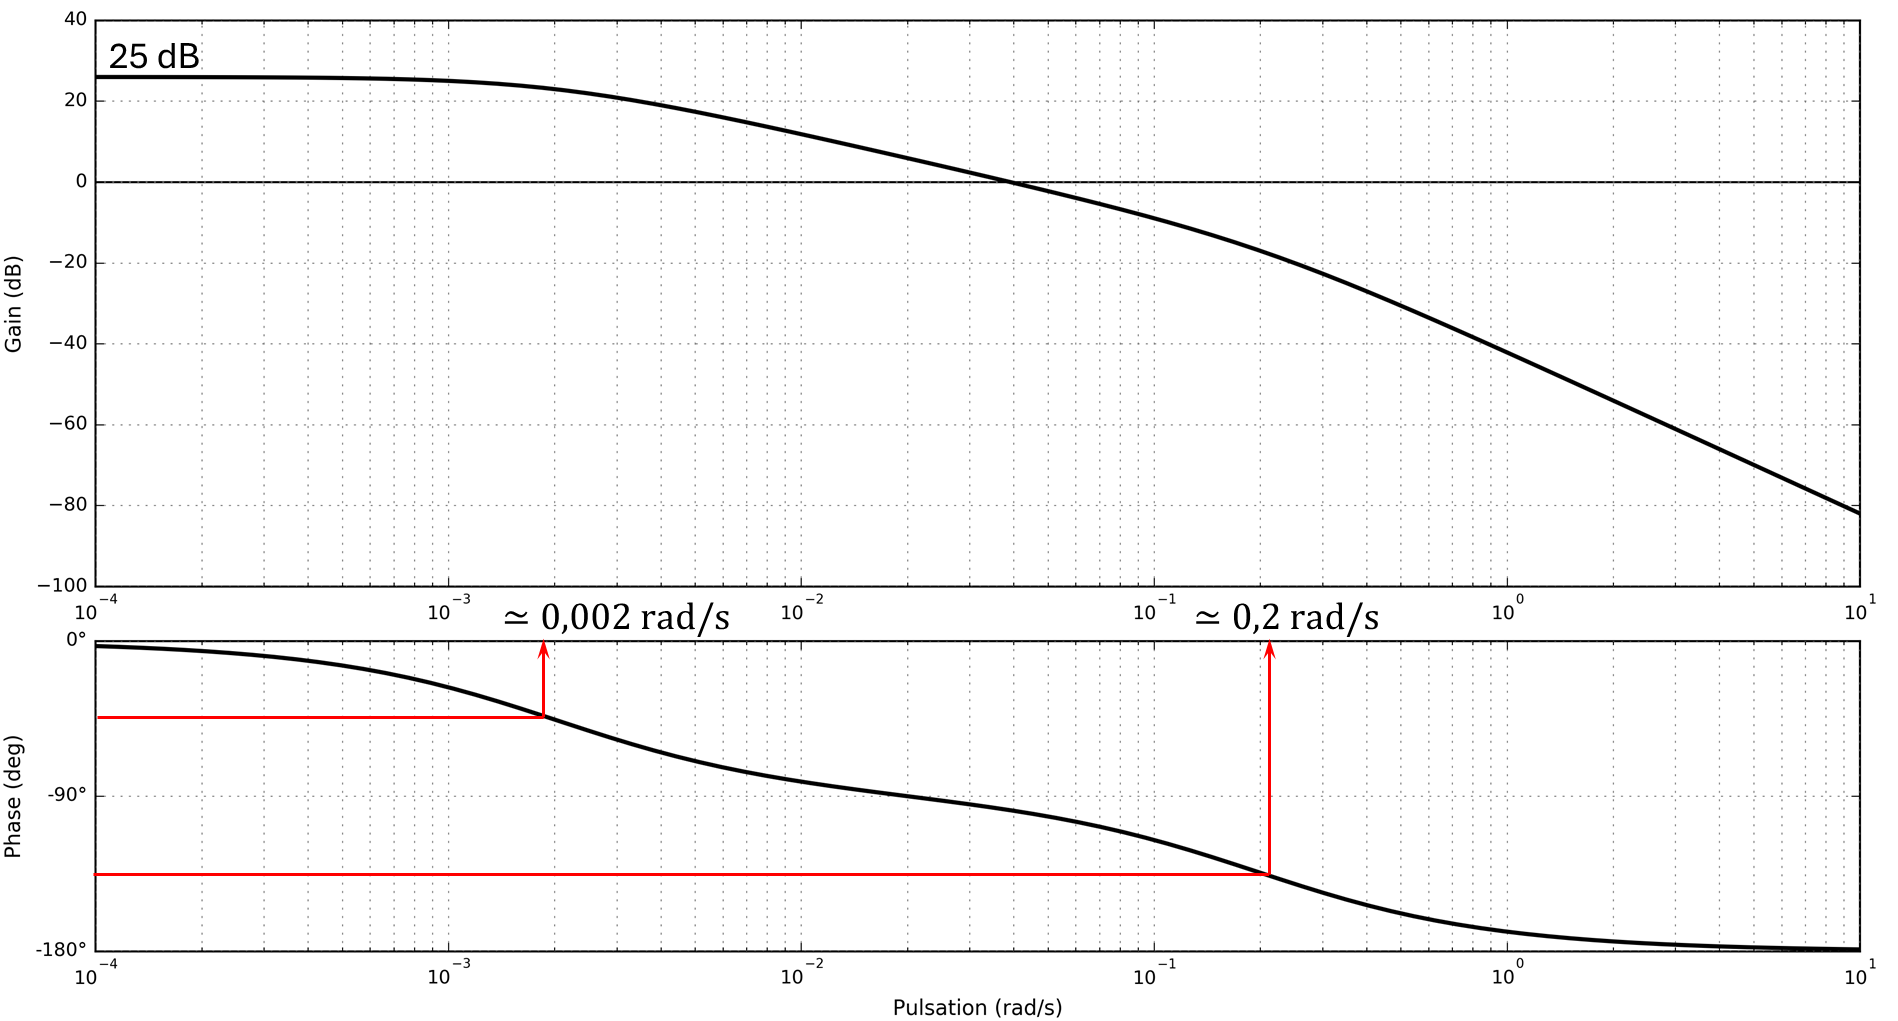
\includegraphics[width=.8\linewidth]{506_01_Cor}
\end{center}
\else
\fi


\ifprof 
\else
Soit la réponse fréquentielle ci-conre \ref{B2:06:506:02:fig}.
\begin{marginfigure}
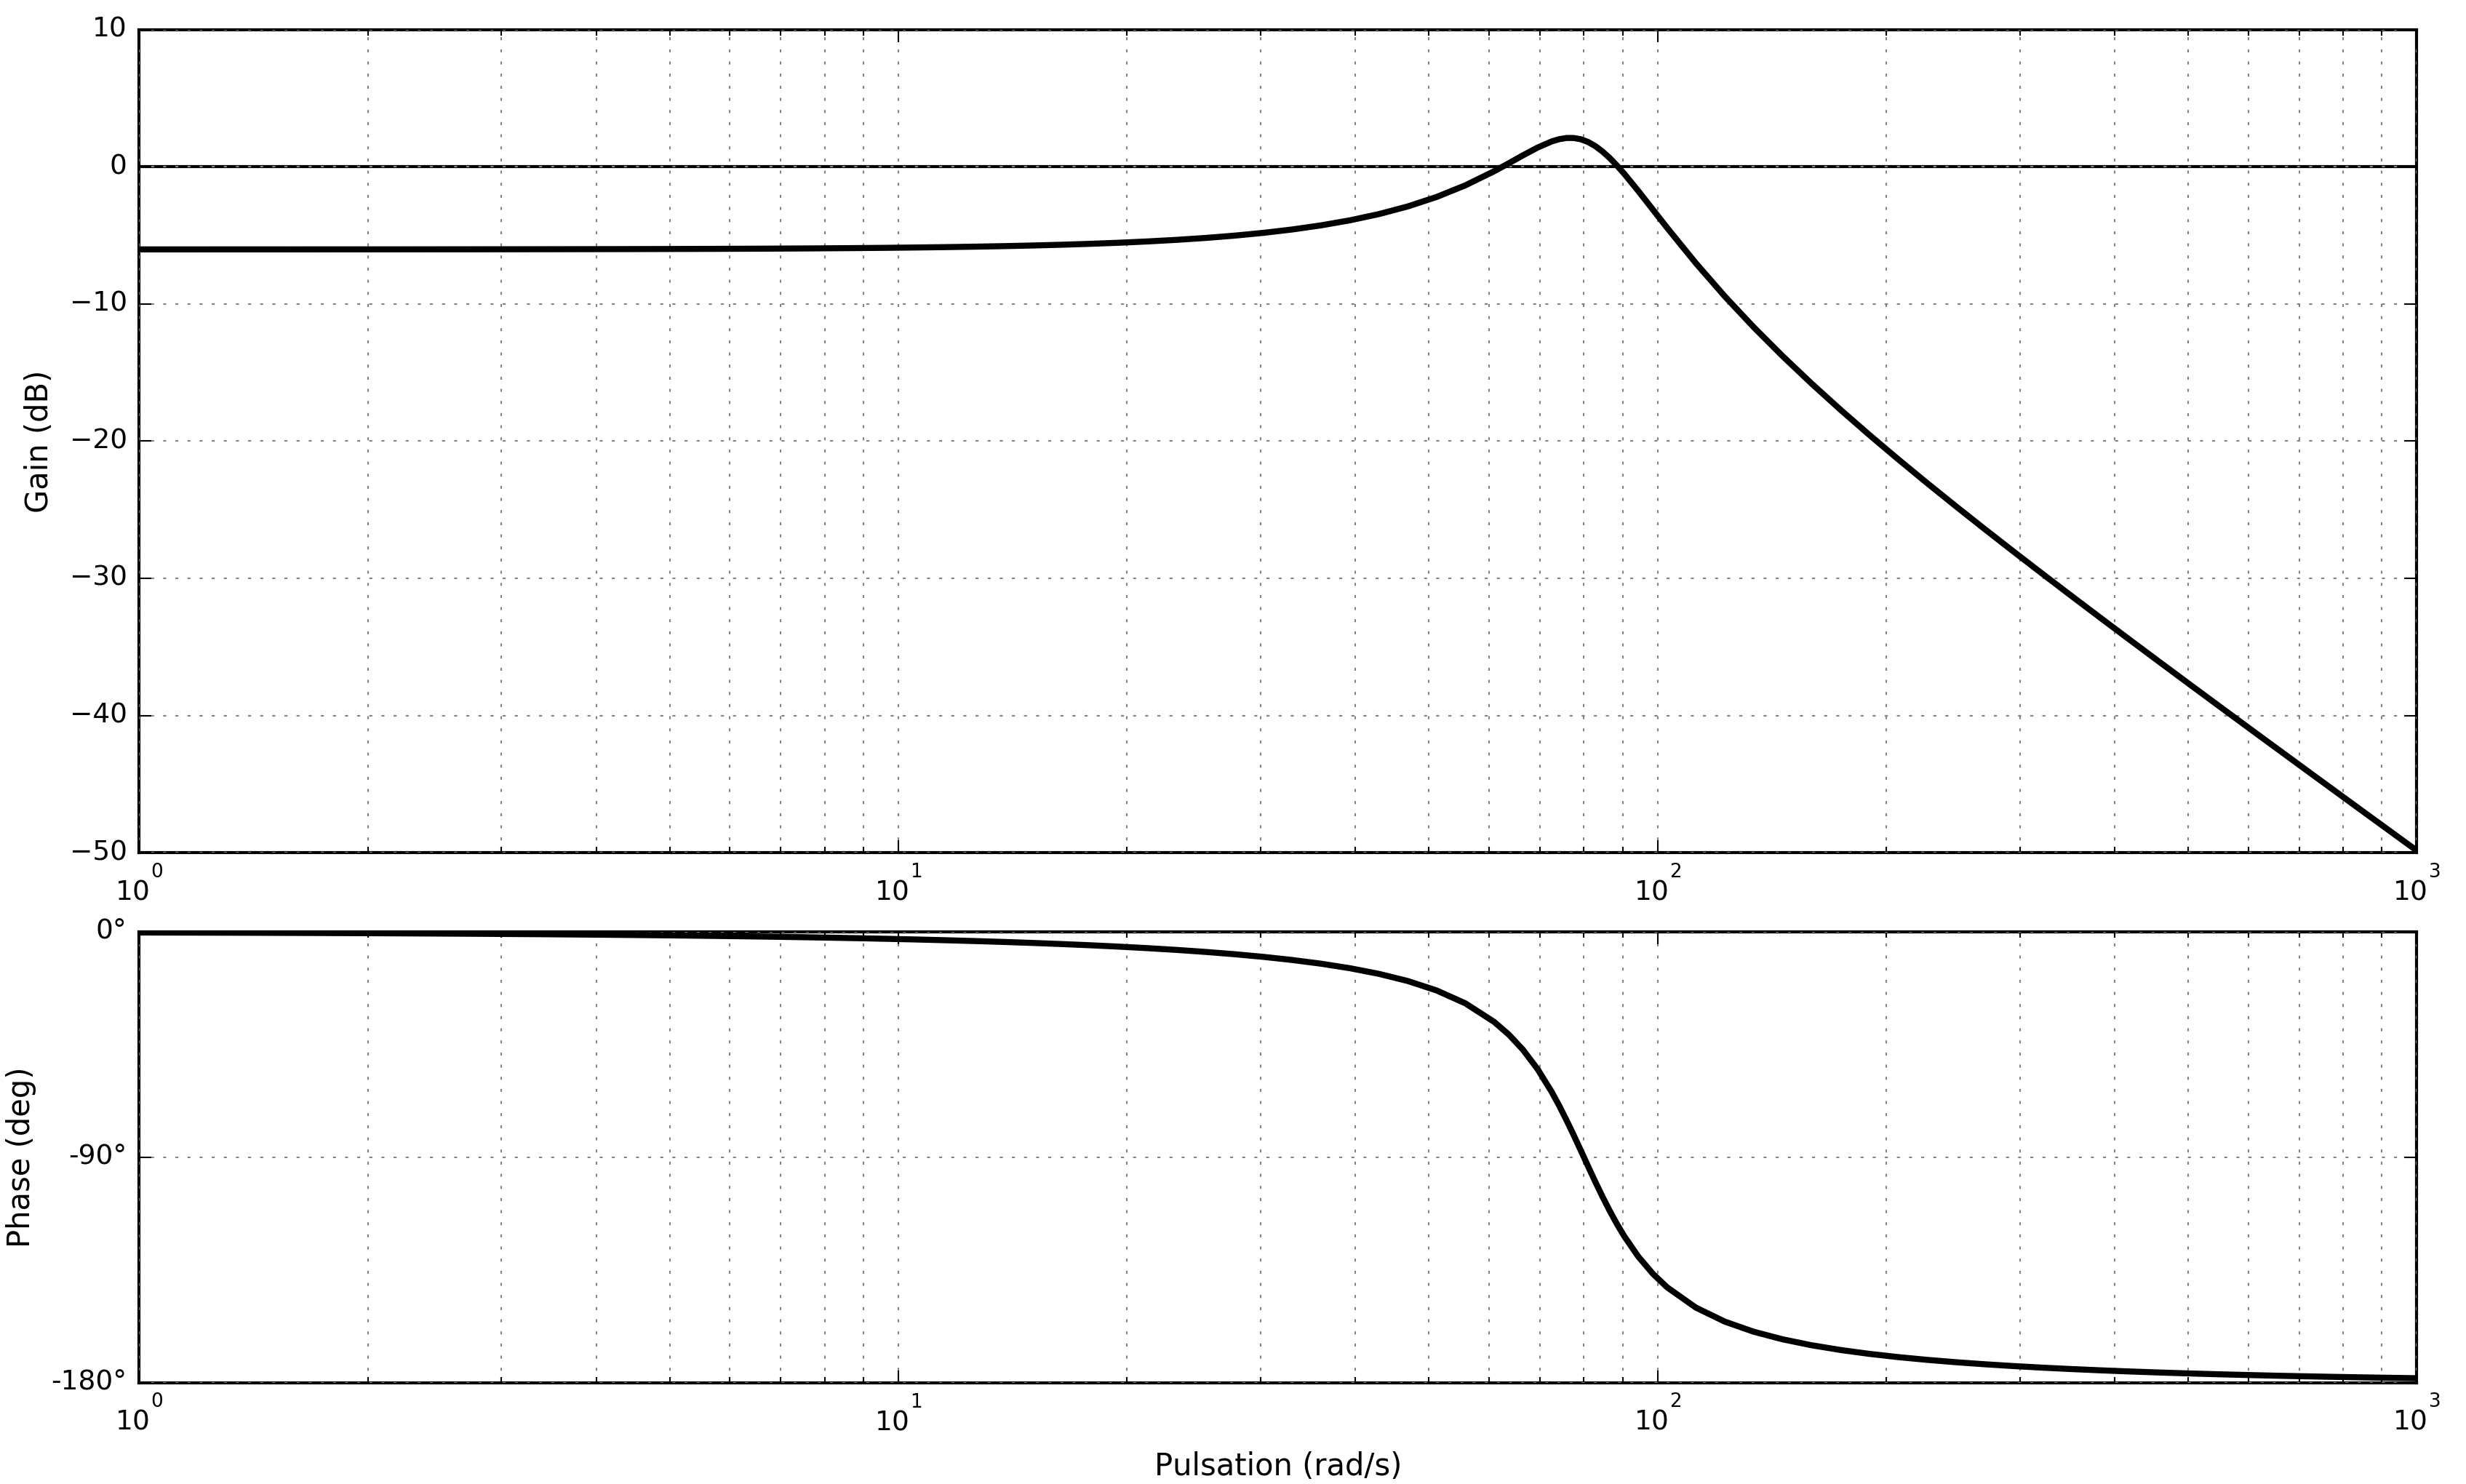
\includegraphics[width=\linewidth]{506_02}
\caption{Diagramme 2 \label{B2:06:506:02:fig}}
\end{marginfigure}
\fi

\question{Déterminer la fonction de transfert du système.}

\ifprof
La phase tend vers 0 en basse fréquence et vers $-180\degres$ en haute fréquence. Le gain tend vers \SI{0}{dB} par décade en basse fréquence et vers $\SI{-40}{dB}$ par décade en haute fréquence.  On observe une résonance. 
On choisit un modèle de la forme $H(p)=\dfrac{K}{1+\dfrac{2\xi}{\omega_0}p+\dfrac{p^2}{\omega_0^2s}}$.

On mesure un gain de $-\SI{-5}{dB}$ en basse fréquence soit $K = 0,56$. 

On mesure $\omega_0 = \SI{80}{rad/s}$ lorsque la phase vaut $-90\degres$.

On mesure un gain de \SI{3}{dB} à la résonance. 
$\xi$ est solution de $10^{(3/20)}\times 2\xi\sqrt{1-x^2}-10^{(-5/20)} = 0$
On trouve $\xi = 0,2$.


\begin{center}
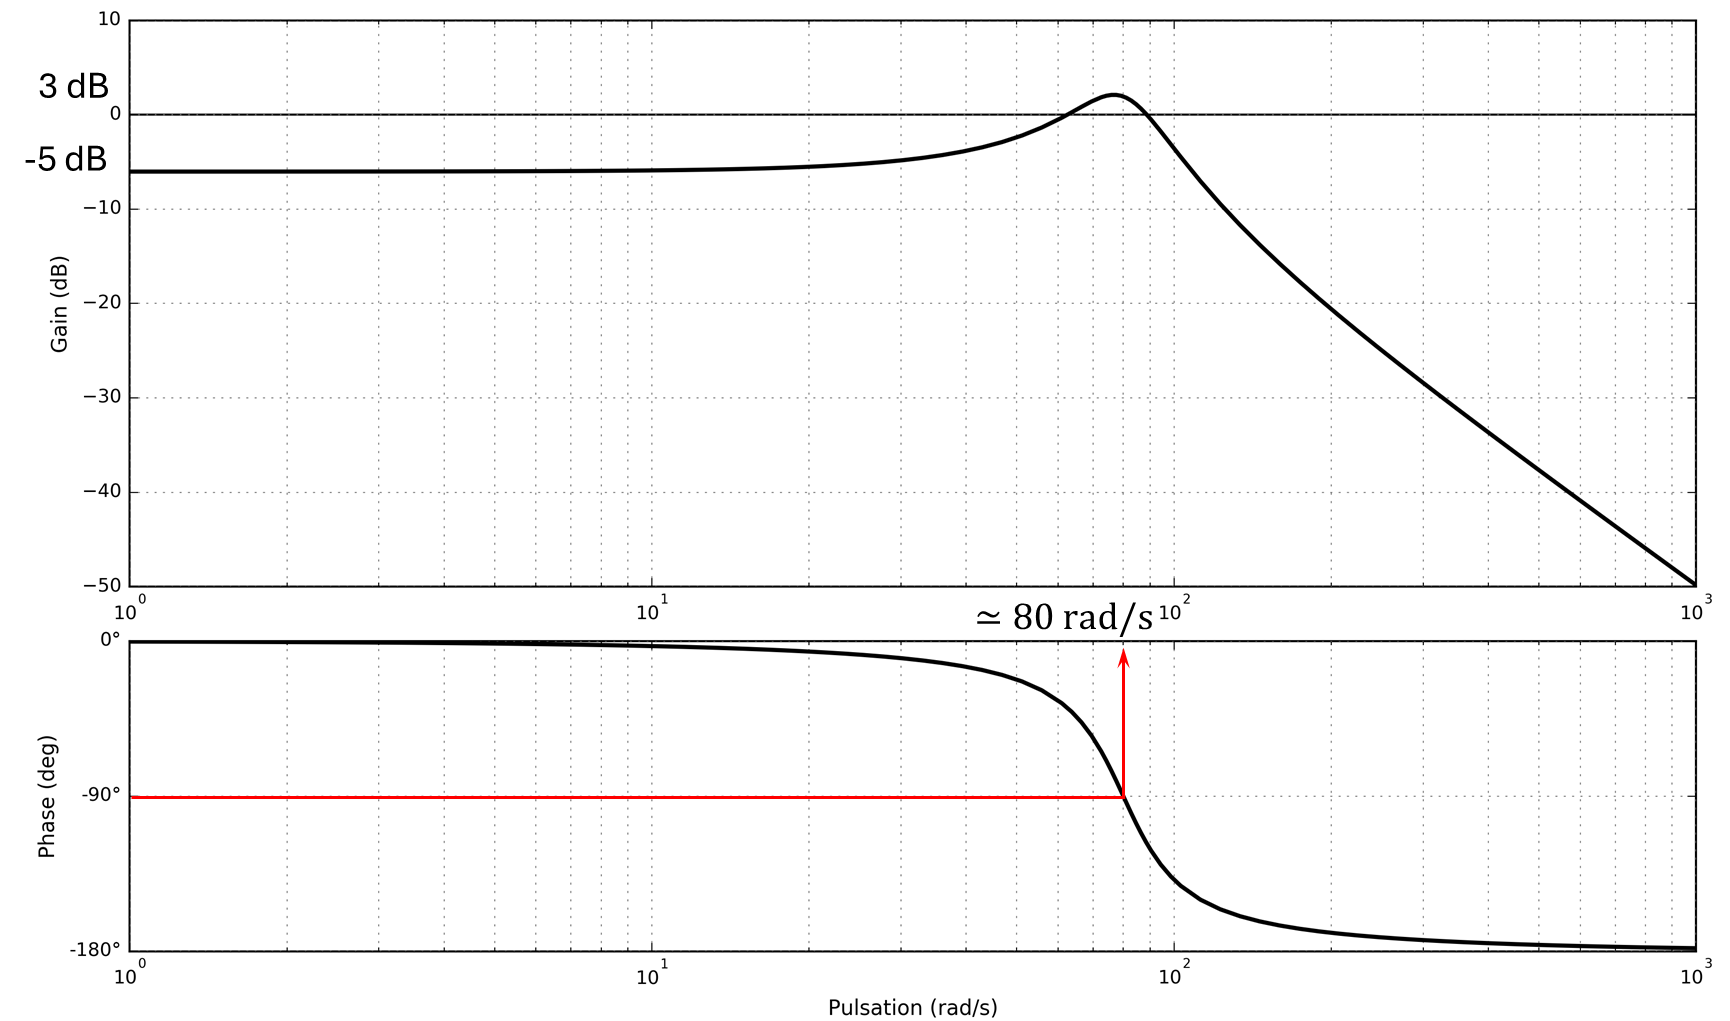
\includegraphics[width=.8\linewidth]{506_02_Cor}
\end{center}

\else
\fi





\ifprof
\else
\marginnote{Corrigé voir \ref{B2:06:506}.}
\fi